\begin{figure*}[th] 
\begin{center}
{\footnotesize
\begin{tabular}{@{}c@{}c@{}c@{}c@{}c@{}c@{}c@{}c@{}} 
\rotatebox{90}{\hspace{3mm}\textbf{(a) Wave 2 }}
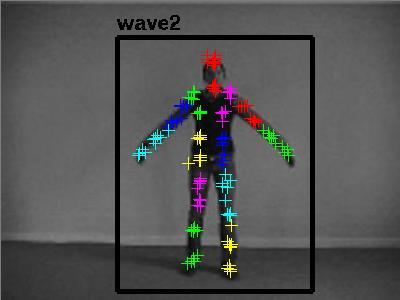
\includegraphics[height=0.11\linewidth]{fig/poseest/others/kth3.jpg} 
&
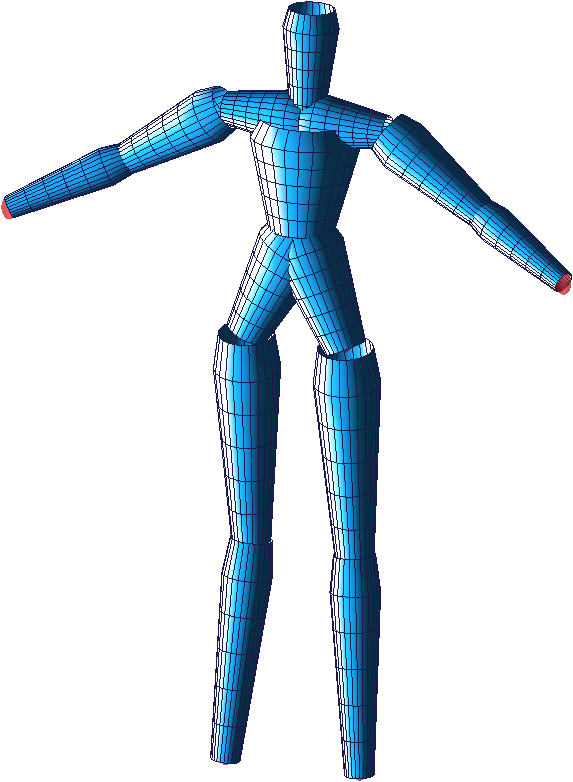
\includegraphics[height=0.135\linewidth]{fig/poseest/others/kth3.png}
& 
\rotatebox{90}{\hspace{3mm}\textbf{(b) Wave 2 }}
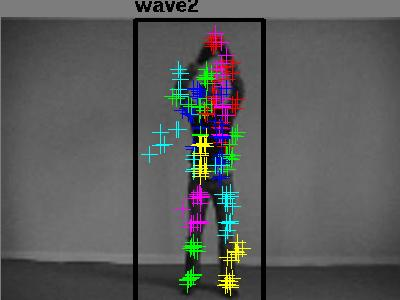
\includegraphics[height=0.11\linewidth]{fig/poseest/others/kth1.jpg} 
&
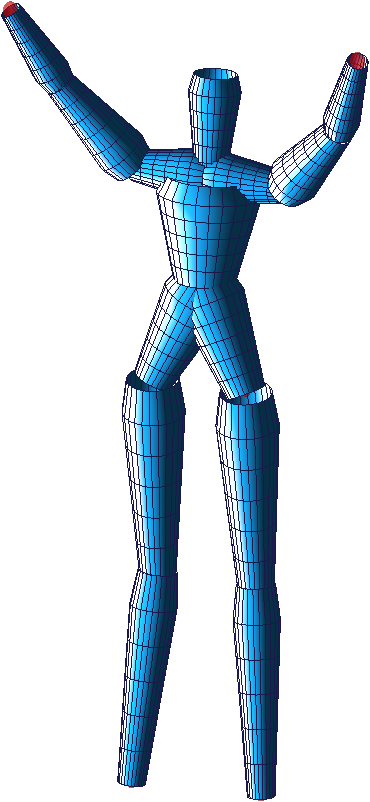
\includegraphics[height=0.135\linewidth]{fig/poseest/others/kth1.png}
& 
\rotatebox{90}{\hspace{3mm}\textbf{(c) Clap }}
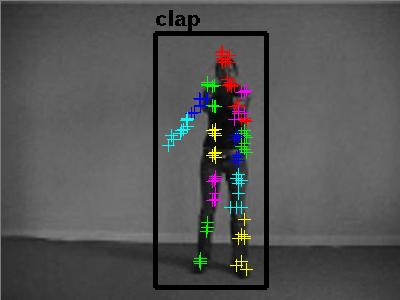
\includegraphics[height=0.11\linewidth]{fig/poseest/others/kth2.jpg} 
&
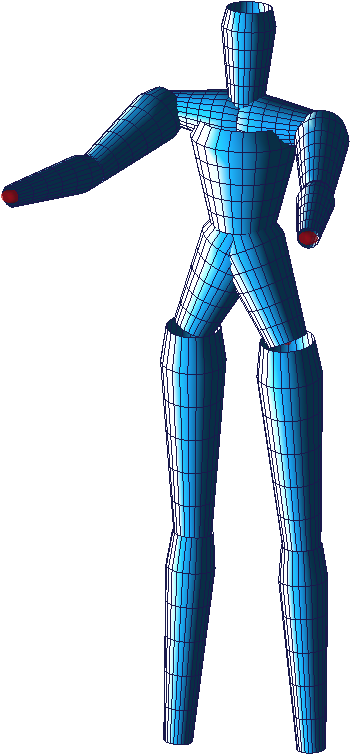
\includegraphics[height=0.135\linewidth]{fig/poseest/others/kth2.png}
& 
\rotatebox{90}{\hspace{3mm}\textbf{(d) Wave 1 }}
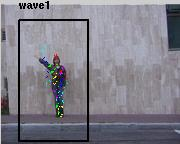
\includegraphics[height=0.11\linewidth]{fig/poseest/others/weiz3.jpg} 
&
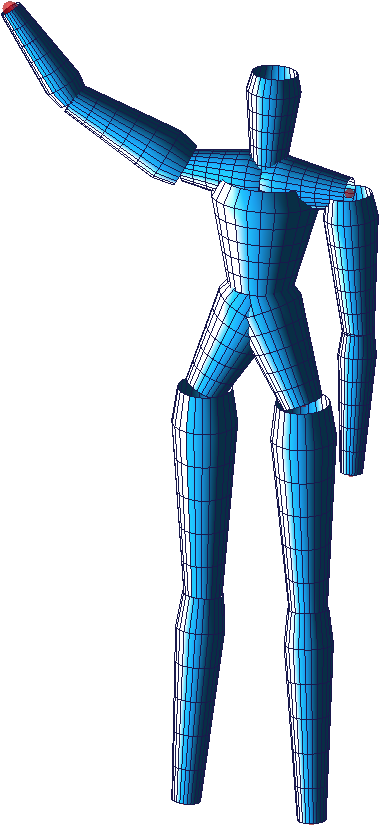
\includegraphics[height=0.135\linewidth]{fig/poseest/others/weiz3.png}
\\
\rotatebox{90}{\hspace{3mm}\textbf{(e) Wave 1 }}
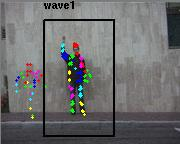
\includegraphics[height=0.11\linewidth]{fig/poseest/others/weiz1.jpg} 
&
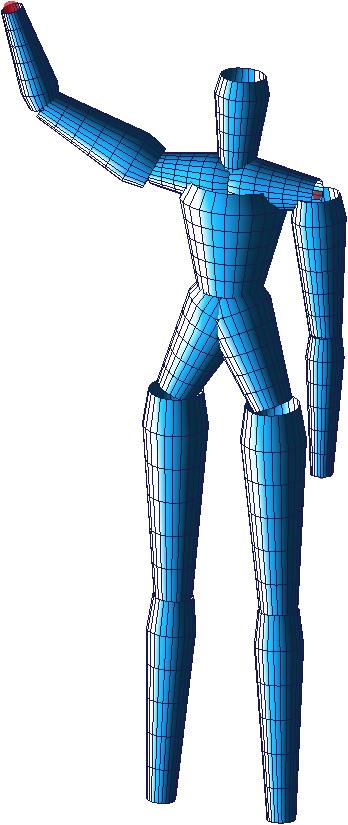
\includegraphics[height=0.135\linewidth]{fig/poseest/others/weiz1.png}
& 
\rotatebox{90}{\hspace{3mm}\textbf{(f) Wave 2 }}
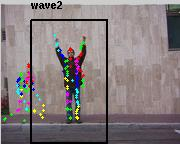
\includegraphics[height=0.11\linewidth]{fig/poseest/others/weiz2.jpg} 
&
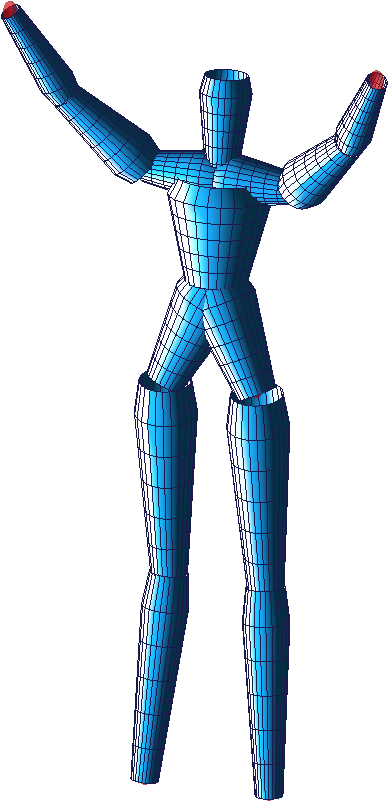
\includegraphics[height=0.135\linewidth]{fig/poseest/others/weiz2.png}
& 
\rotatebox{90}{\hspace{3mm}\textbf{(g) Wave 2 }}
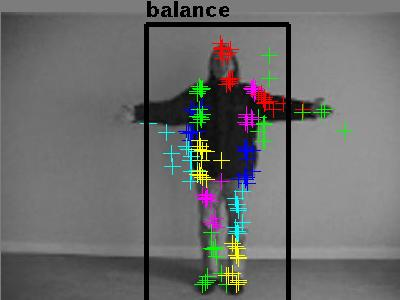
\includegraphics[height=0.11\linewidth]{fig/poseest/others/ktherr.jpg} 
&
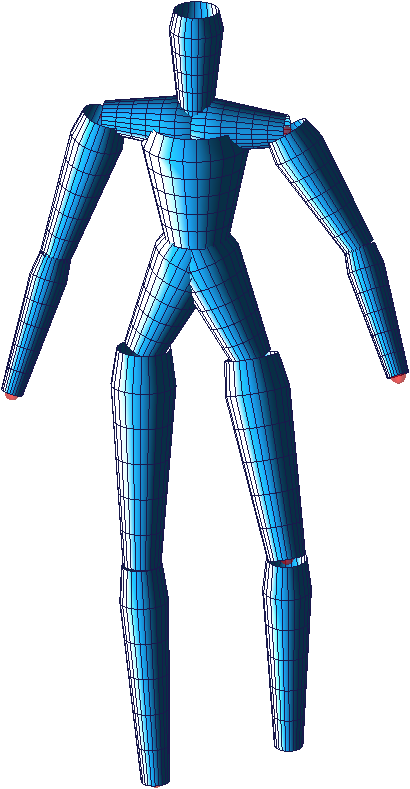
\includegraphics[height=0.135\linewidth]{fig/poseest/others/ktherr.png}
& 
\rotatebox{90}{\hspace{3mm}\textbf{(h) Wave 1 }}
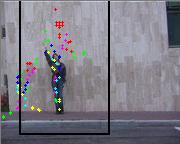
\includegraphics[height=0.11\linewidth]{fig/poseest/others/weizerr.jpg} 
&
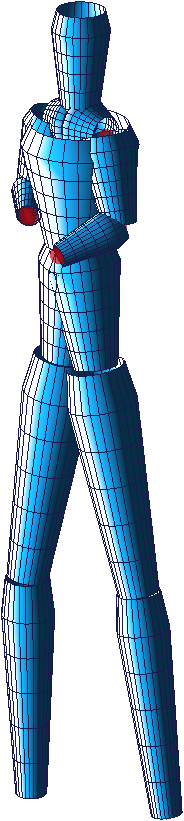
\includegraphics[height=0.135\linewidth]{fig/poseest/others/weizerr.png}
\end{tabular}
\caption{Sample results obtained from applying the same model trained in Section \ref{sec:quant} to KTH (a--c, g) and Weizmann dataset (d--f, h).} 
\label{fig:otherresults}
} 
\end{center} 
\end{figure*} 
